\section{Result II: The Information Gap Is in Convolution on the MXU}
\label{sec:result2}

\subsection{The remaining error is concentrated on convolution graphs}
\label{sec:conv-error}
Ranking errors pile up on convolution graphs (Figure~\ref{fig:conv}). On xla:random's 7 validation
graphs, averaging the flat and contention-edge models over five seeds at the shared lr, the top-ranked
layout is 1.44--1.51$\times$ slower than the best on the three convolution-dominated graphs, against
1.01--1.07$\times$ on the other four (UNet-3D and three BERT variants, which are memory- or
matmul-bound). At evaluation batch 8 the ranges are 1.21--1.52$\times$ and 1.01--1.08$\times$, so every
convolution graph is still worse than every other graph. The grouping was chosen after seeing the
results, so it is exploratory; the rest of this section tests it without models.

\begin{figure}[t]
\centering
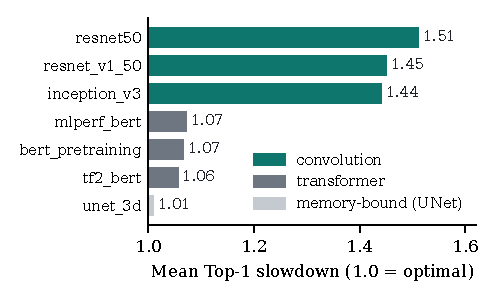
\includegraphics[width=\columnwidth]{figures/fig_c1_conv_failure.pdf}
\caption{Per-graph Top-1 slowdown on xla:random's validation graphs, averaged over the flat and
contention-edge models and five seeds (shared lr 1e-3, evaluation batch 32; 1.0 = optimal). The three
convolution graphs are 44--51\% slower than the best layout; the others are 1--7\% slower.}
\label{fig:conv}
\end{figure}

\subsection{Measured runtimes alone show the gap}
\label{sec:model-free}
For each graph--collection pair we computed the spread of measured runtimes across layouts
(coefficient of variation). The median spread is 0.239 across 95 convolution-bearing pairs against
0.086 across 49 convolution-free pairs: convolution-bearing graphs vary 2.77 times as much
(Mann--Whitney $p = 1.5\times10^{-7}$). Across all 144 pairs, the share of a graph's compute that runs
on the MXU correlates with its runtime spread (Spearman $\rho = +0.52$). A model that ranks convolution
graphs poorly therefore faces a harder problem, not merely a failure of prediction.

\subsection{The physical reason}
\label{sec:physical}
In the 4 convolution-bearing validation graphs, every convolution has an arithmetic intensity between
90 and 2,900 FLOPs/byte, all above the TPU v3 ridge. Every convolution is therefore compute-bound, and
its runtime is set by how efficiently its tiling uses the MXU. A layout change can alter the tiling and
with it the padding waste and the speed, and that tiling is exactly what the graph does not record.
\TODO{FACT ERROR, fix in your words: erratum 9648419 (2026-10-13) says NOT every conv is above the
ridge. Per op, 11--26\% of conv ops are below 137 FLOP/byte (1--16\% of MACs); per-op intensity spans
3.8--11,810. Correct claim: conv work is predominantly compute-bound (74--89\% of ops, 84--99\% of MACs;
MAC-weighted intensity 688--2,857). Source: experiments/phase8_mxu_misalignment.md, Erratum.}

\subsection{Three simple static explanations fail}
\label{sec:static-fail}
% REVISE-IF-TIME: low 4-gram overlap with the First Draft.
If the sensitivity could be read off simple static summaries, a model should not need the compiler's
tiling. Three such summaries fail. (a)~Channel-padding waste does not predict runtime spread across
convolution graphs ($\rho = -0.06$, $n = 95$, $p = .53$): no detectable correlation. (b)~Roofline
position does not order failure: UNet-3D, the most MXU-intense graph (intensity $\approx$ 2,857), is
handled best at 1.01$\times$, while the failing graphs sit near 690--730 (Inception 1.44$\times$,
ResNet-v1-50 1.45$\times$, ResNet-50 1.51$\times$). (c)~Within-convolution MXU overhead runs opposite
to slowdown: Inception has the highest overhead (1.69) and the lowest slowdown of the three, the
ResNets the lowest (1.17) and the highest. Checks (b) and (c) are illustrations on 4 and 3 graphs, not
tests.

This does not contradict Section~\ref{sec:capstone}. Here we ask a between-graph question: does a
graph's average padding waste predict its runtime spread? Section~\ref{sec:capstone} asks a
within-graph one: does per-node MXU geometry, given to the model, help rank configurations inside a
graph? Our explanation for the gap, that the graph omits the compiler's tiling choice, is inferred from
these results; we did not observe that choice directly.
